%% A "teaser" image appears between the author and affiliation
%% information and the body of the document, and typically spans the
%% page.
\begin{teaserfigure}
    \subfloat[]{
    \label{fig:teaser:a}
    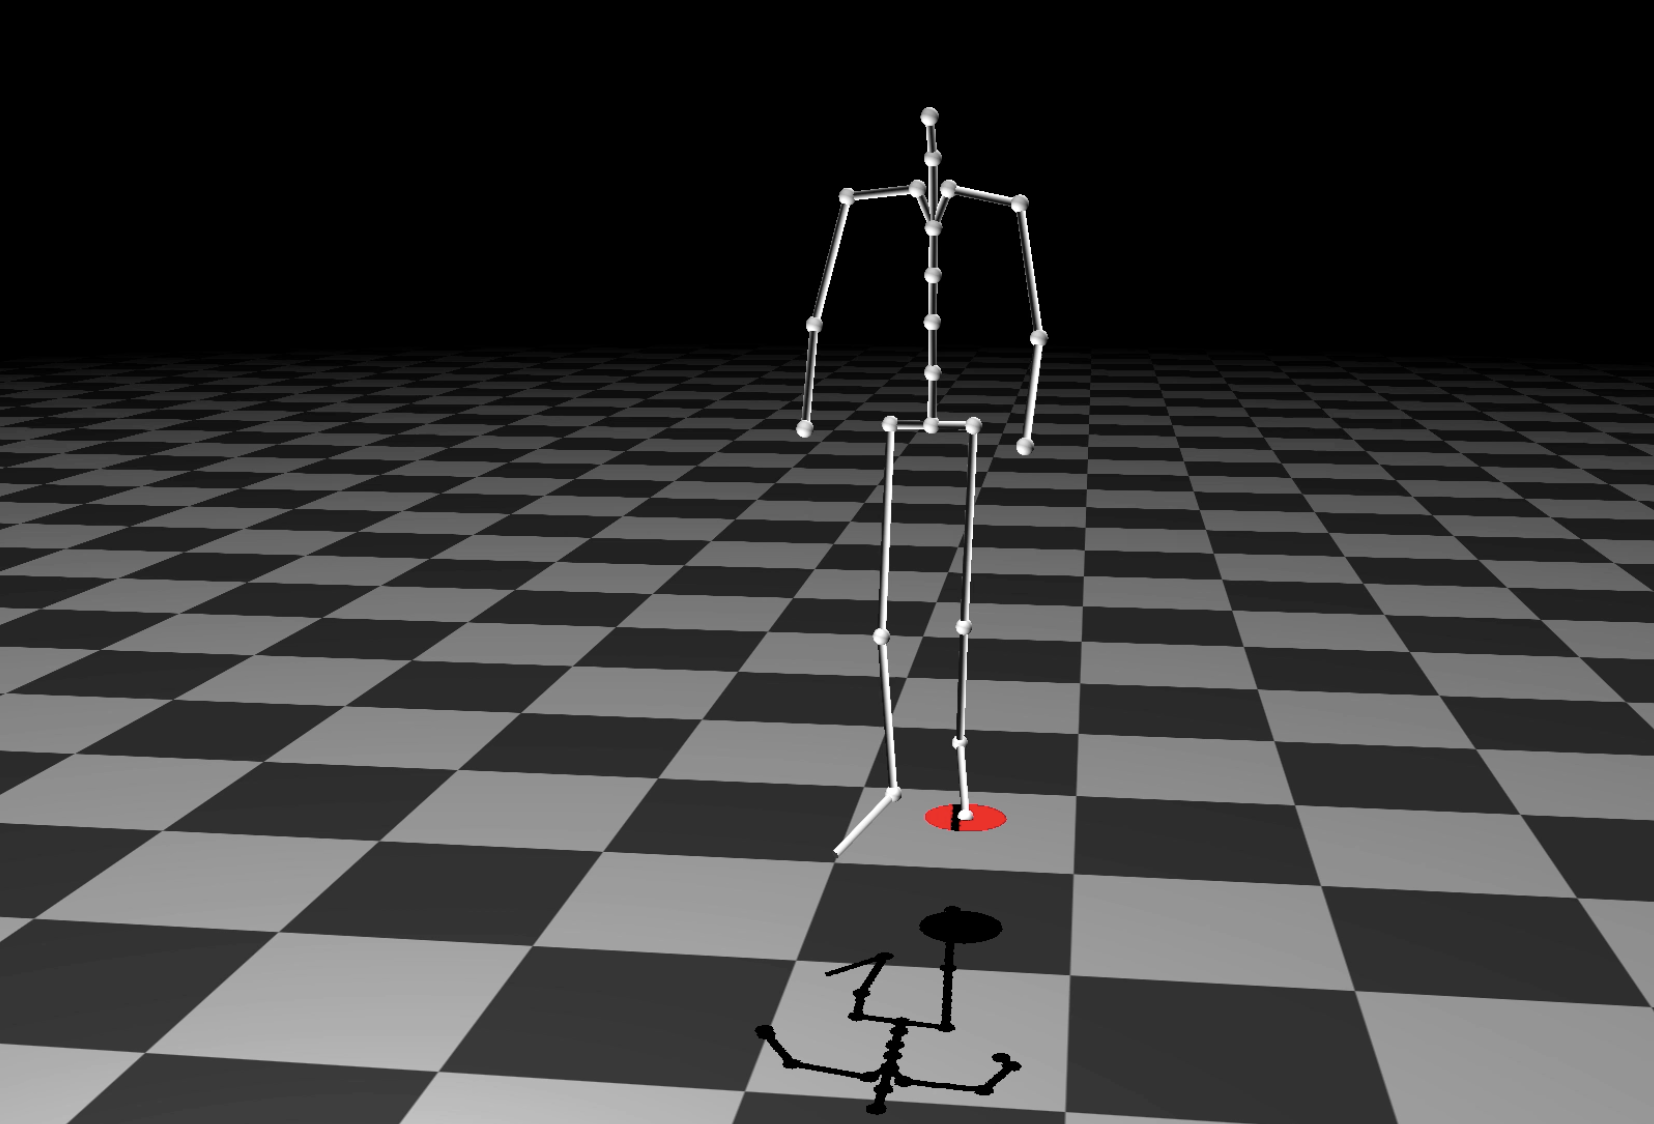
\includegraphics[width=1\textwidth]{img/teaser}
    }
    \protect \caption{
    \kenny{Teaser might look more cool if we can make one long horizontal time-lapse showing the character going from left to right in a zig-zag like pattern? You almost got this. Might be good if we could have two rows, top row using our method, bottom row with state-of-the-art practice in games?}
    Our Movement models provide both a weak control signal for interactive games as well as accurate description of the actual motion. The model can be auto-tuned and generated from data offline to generate fluent and consistent motion as seen above.} 
  \Description{Awesome.}
  \label{fig:teaser}
\end{teaserfigure}
